%%%%%%%%%%%%%%%%%%%%%%%%% PREAMBLE %%%%%%%%%%%%%%%%%%%%%%%%%%%%%%%%
\documentclass[a4paper]{article}
\usepackage[utf8]{inputenc}
\usepackage{longtable}
\usepackage{array}
\usepackage{booktabs}
\usepackage{multirow}
\usepackage{rotating}
\usepackage[font=small,labelfont=bf]{caption}
\usepackage{subcaption}
\usepackage[]{natbib}
\bibliographystyle{apalike}
\usepackage{geometry}
\geometry{a4paper,total={150mm},left=30mm,right=30mm,top=30mm,bottom=30mm}
\usepackage{graphicx}
\usepackage{adjustbox}
\graphicspath{{/images/}}
%%%%%%%%%%%%%%%%%%%%%%%%%%%%%%%%%%%%%%%%%%%%%%%%%%%%%%%%%%%%%%%%%%%%%

\begin{document}
\title{Final Project (1653 words)}
\author{Di Zhen (1717719)}
\date{\today}
\maketitle
\newpage

\section*{Introduction}

Suicide has drawn a primary public health concern in China. There are about 13 deaths per 100,000 people commit suicide each year. The features of suicide in China are important and unique. They are different from the features in the western world. In China, women are more likely to commit suicide than men \citep{ChenZReportontheThird}. The elderly have a higher suicide rate than the young \citep{PhillipsMR}. People living in rural areas commit more suicide than those in urban \citep{YangGH}. And pesticide self-poisoning has been reported to be the main suicide method \citep{AjdacicGrossV}. In addition, suicide actions not only result in loss of lives but also cause hospitals to suffer from a tremendous burden on resources, since the majority of people who committed suicide are survived and hospital-admitted.
\newline
\newline
The study of fatal suicide attempts in China would indicate factors leading to a fatal outcome after a suicide attempt, and also give suggestions about the prevention of suicide acts. In this report, we replicate part of the surveillance study \citep{Sun2015} on the incidence and fatality of serious suicide attempts (SSA) in Shandong, China. 

\section*{Methods}

The data are from two public health surveillance system, which are the Disease Surveillance Points (DSP) system and Shandong Injury Surveillance System (ISS). The authors in the surveillance study \citep{Sun2015} extracted data of suicide deaths and hospitalizations in three selected cities in Shandong, China and ascertained the cases by the 10th revision of the International Classification of Diseases and Related Health Problems.
\newline
\newline
After categorizing and cleaning the data, there are 2289 people and 8 major variables including whether dead or not, living in urban or rural areas, sex, age group, education level, occupation, method of suicide, and season of suicide. The age group includes 10-34, 35-49, 50-64, and no less than 65. The education level includes illiterate, primary, and no less than secondary level (secondary and tertiary). The occupation includes farming and all others(household, professional, unemployed, business, student, worker, retiree, others). The methods of suicide include hanging, pesticide, other poison(other poison, unspecified poison), and all others(cutting, drowning, jumping, others). The season is defined as spring(March-May), summer(June-August), autumn(September-November) and winter(December-February).
\newline
\newline
Fatality rate(\%) is the proportion of died cases among all SSAs. $\chi^2$ test was conducted to test the differences in fatality between groups and p-values were reported. Multiple logistic regression was also applied to test the associations between main factors and fatality, and the ORs, 95\% CIs and p-values were reported. In order to extend the analysis of the authors', the assumption of multiple logistic regression mentioned above was tested. In addition, the data were grouped by residency, sex, age group, education, occupation, method, and season.Then, the number of death for each group was counted. Using this grouped data, a Poisson regression was conducted to analyze the associations between main factors and fatality, and the assumption of the Poisson regression was tested subsequently. All statistical analyses were conducted in R (Version 3.6.3).

\section*{Results and Discussion}

As shown in Table \ref{tab:T1}, people who are living in a urban area, who are male, who are older, who are with low education, or with a farmer occupation have higher fatality rates (all chi-square test, p-value < 0.05). As for the suicide methods, the fatality of using other poison (10.0\%) is the lowest, while the fatality of hanging (97.4\%) is the highest. Attempts in seasons other than summer have higher fatality rates. The p-values of chi-square test are all less than 0.05, indicating that those independent variables are significantly associated with the fatality.
\newpage
% replicate Table 3

\begin{table}[!htbp]
%\centering
%\begin{tabular}{|*{6}{c|}}
\begin{tabular}[c]{@{}>{\raggedright\arraybackslash}p{35mm}>{\raggedright\arraybackslash}p{18mm}p{23mm}p{15mm}p{30mm}p{15mm}@{}}
\toprule
 \multicolumn{1}{c}{\textbf{~}} &
 \multicolumn{3}{|c}{\textbf{Bivariate analysis}} & \multicolumn{2}{|c}{\textbf{Multiple logistic regression}} \\ \midrule


 & \textbf{Number of SSAs)} &
 \textbf{Fatality(\%)} &
 \textbf{p Value$^1$} &
 \textbf{OR(95\%~CI)} &
 \textbf{p Value$^2$} \\ \midrule

\textbf{\textit{Residency}} & ~  & ~ & ~ & ~ & ~  \\
\textbf{\textit{~~~~Rural}} & 2064  & 1125 (54.5) & 0.047  & 1.00  & Reference  \\
\textbf{\textit{~~~~Urban}} & 225  & 107 (47.6) & ~  & 1.18 (0.82, 1.68)  & NS  \\


\textbf{\textit{Sex}} & ~  & ~ & ~ & ~ & ~  \\
\textbf{\textit{~~~~Female}} & 1184 & 579 (49.0) & < 0.001  & 1.00  & Reference  \\
\textbf{\textit{~~~~Male}} & 1105 & 653 (59.1) & ~  & 1.30 (1.04, 1.62)  & 0.02 \\  

\textbf{\textit{Age group}} & ~  & ~ & ~ & ~ & ~  \\
\textbf{\textit{~~~~10-34}} & 482 & 117 (24.3) & < 0.001  & 1.00  & Reference \\ 
\textbf{\textit{~~~~35-49}} & 488 & 187 (38.3) & ~  & 1.33 (0.97, 1.83)  & NS \\ 
\textbf{\textit{~~~~50-64}} & 569 & 337 (59.2) & ~  & 1.59 (1.14, 2.22)  & 0.007 \\  
\textbf{\textit{~~~~65 and above}} & 750 & 591 (78.8) & ~  & 2.13 (1.47, 3.07)  & <0.001   \\  


\textbf{\textit{Education}} & ~  & ~ & ~ & ~ & ~  \\
\textbf{\textit{~~~~Secondary and above}} & 1136 & 317 (27.9) & < 0.001 & 1.00 & Reference \\  
\textbf{\textit{~~~~Primary}} & 633 & 463 (73.1) & ~ & 4.77 (3.63, 6.31)  & <0.001 \\ 
\textbf{\textit{~~~~Illiterate}} & 520 & 452 (86.9) & ~ & 10.93 (7.65, 15.83)  & <0.001  \\


\textbf{\textit{Occupation}} & ~  & ~ & ~ & ~ & ~  \\
\textbf{\textit{~~~~All Others}} & 355 & 150 (42.3) & < 0.001 & 1.00  & Reference \\
\textbf{\textit{~~~~Farming}} & 1934 & 1082 (55.9) & ~ & 1.35 (0.98, 1.86)  & NS \\


\textbf{\textit{Method}} & ~  & ~ & ~ & ~ & ~  \\
\textbf{\textit{~~~~Pesticide}} & 1645 & 761 (46.3) & <0.001 & 1.00  & Reference \\
\textbf{\textit{~~~~Other poison}} & 160 & 16(10.0) & ~ & 0.09 (0.05, 0.16)  & <0.001 \\
\textbf{\textit{~~~~Hanging}} & 420 & 409 (97.4) & ~ & 26.79 (14.99, 53.17) & <0.001 \\
\textbf{\textit{~~~~All others}} & 64 & 46 (71.9) & ~ & 3.70 (2.00, 7.04) & <0.001 \\


\textbf{\textit{Season}} & ~  & ~ & ~ & ~ & ~  \\
\textbf{\textit{~~~~Summer}} & 669 & 316 (47.2) & <0.001 & 1.00  & Reference \\
\textbf{\textit{~~~~Autumn}} & 558 & 287 (51.4) & ~ & 1.11 (0.83, 1.49) & NS \\
\textbf{\textit{~~~~Winter}} & 473 & 278 (58.8) & ~ & 1.65 (1.20, 2.26) & 0.002 \\
\textbf{\textit{~~~~Spring}} & 589 & 351 (59.6) & ~ & 1.65 (1.23, 2.21) & <0.001 \\


\bottomrule
\end{tabular}
\footnotesize{$^1$Test the differences in fatality between groups using Chi-square test.}\\
\footnotesize{$^2$Test for regression coefficients in the multiple logistic model.}\\
\footnotesize{NS, not signficant (p>0.05); SSA, serious suicide attempts.}\\
\caption{Fatality (\% and 95\% CIs) of SSAs and results of multiple logistic regression analysis (ORs and 95\% CIs).}
\label{tab:T1} \\
\end{table}

The result of multiple logistic regression is summarized in Table \ref{tab:T1}. People living in urban have a 18\% increase in the odds of death by suicide compared to those living in rural areas, after controlling for sex, age group, education, occupation, method, and season. Males have a 30\% increase in the odds of death by suicide compared to female after controlling for other variables. Those in the age group of 35-49, 50-64, and 65 and above have ORs of 1.33, 1.59, and 2.13 for death due to suicide versus being alive compared to those in the age group 10-34, after controlling for other variables. People with primary and illiterate educational level have a 377\% and 993\% increase in the odds of death due to suicide compared to those with secondary and above educational level, after controlling for other variables. People who are farmer have a 35\% increase in the odds of death due to suicide compared to those with vocations other than farming, after controlling for other variables. Those hanging and using other methods to commit suicide have a 2579\% and 270\% increase in the odds of death due to suicide compared to those using pesticides, after controlling for other variables. While those using other poison have a 91.0\% decrease in the odds of death due to suicide compared to those using pesticides, after controlling for other variables. People committing suicide in autumn, winter and spring have a 11\%, 65\%, and 65\% increase in the odds of death due to suicide compared to those committing suicide in summer, after controlling for the other variables. The p values of urban residency, 10-34 age group, Farming, and suicide in autumn are not significant, while others are significant (p-value > 0.05).
\newline
% Poisson Regression
\begin{table}[!htbp]
\centering
\begin{tabular}[c]{@{}lll@{}}
\toprule
 & \multicolumn{2}{c}{\textbf{Poisson Regression}} \\* \midrule

\textbf{~}  & \textbf{OR(95\% CI)}& \textbf{p Value*} \\ \midrule

\textbf{\textit{Residency}} & ~ & ~   \\
\textbf{\textit{~~~~Rural}} & 1.00 & Reference   \\
\textbf{\textit{~~~~Urban}} & 0.21 (0.17, 0.26) & <0.001  \\

\textbf{\textit{Sex}}  & ~ & ~ \\
\textbf{\textit{~~~~Female}} & 1.00 & Reference   \\
\textbf{\textit{~~~~Male}} & 1.09 (0.97, 1.22) & NS \\  

\textbf{\textit{Age group}} & ~ & ~ \\
\textbf{\textit{~~~~10-34}} & 1.00 & Reference  \\ 
\textbf{\textit{~~~~35-49}} & 1.19 (0.94, 1.50) & NS \\ 
\textbf{\textit{~~~~50-64}} & 1.68 (1.36, 2.08) & <0.001 \\
\textbf{\textit{~~~~65 and above}} &  2.84 (2.33, 3.50) & <0.001 \\

\textbf{\textit{Education}} & ~ & ~ \\
\textbf{\textit{~~~~Secondary and above}} & 1.00 & Reference \\  
\textbf{\textit{~~~~Primary}} & 1.38 (1.20, 1.60) & <0.001 \\ 
\textbf{\textit{~~~~Illiterate}} & 1.48 (1.28, 1.72)& <0.001 \\

\textbf{\textit{Occupation}} & ~ & ~ \\
\textbf{\textit{~~~~All Others}} & 1.00 & Reference \\
\textbf{\textit{~~~~Farming}} & 3.73 (3.15, 4.45) & <0.001 \\

\textbf{\textit{Method}} & ~ & ~  \\
\textbf{\textit{~~~~Pesticide}} & 1.00 & Reference  \\
\textbf{\textit{~~~~Other poison}} & 0.04 (0.02, 0.07) & <0.001 \\
\textbf{\textit{~~~~Hanging}} & 0.75 (0.66, 0.85) & <0.001 \\
\textbf{\textit{~~~~All others}} & 0.20 (0.15, 0.27) & <0.001 \\

\textbf{\textit{Season}} & ~ & ~  \\
\textbf{\textit{~~~~Summer}} & 1.00 & Reference \\
\textbf{\textit{~~~~Autumn}} & 0.96 (0.82, 1.13) & NS \\
\textbf{\textit{~~~~Winter}} & 0.97 (0.82, 1.14) & NS \\
\textbf{\textit{~~~~Spring}} & 1.31 (1.12, 1.52) & <0.001 \\* 
\bottomrule

\end{tabular}

\footnotesize{*Test for regression coefficients in the Poisson regression model.}\\
\footnotesize{NS, not signficant (p>0.05); SSA, serious suicide attempts.}\\
\caption{Results of Poisson regression analysis (ORs and 95\% CIs)}
\label{tab:T2}
\end{table}

\newline
The result of a Poisson regression is summarized in Table \ref{tab:T2}. Compared to people living in rural areas, those in urban have a 79\% decrease in fatality rate after controlling for sex, age group, education, occupation, method, and season. Compared to females, males have a 9\% increase in fatality rate after controlling for other variables. Compared to those in the age group of 10-34, people in the age group of 35-49, 50-64, and 65 and more age groups have 19\%, 68\%, and 184\% increase respectively in fatality rate, after controlling for other variables. Compared to those with secondary and above education, people with primary and illiterate education have 38\% and 48\% increase respectively in fatality rate after controlling for other variables. Compared to people with occupations other than farmers, those farmers have a 273\% increase in fatality rate after controlling for other variables. Compared to people using pesticides to commit suicide, those using other poison, hanging, and using other methods have 96\%, 25\%, and 80\% decrease respectively in fatality rate, after controlling other variables. Compared to cases in summer, those who suicide in autumn, winter, and spring have 4\%,  3\% decrease and, 31\% increase respectively in fatality rate, after controlling for other variables. The p-values of male, age group of 35-49, suicide in autumn and winter are not significant(p-value >0.05), while others are statistically significant.
\newline
\newline
The result of multiple logistic regression and Poisson regression is slightly different. Most of the CIs of variables in multiple logistic regression are wider than those in Poisson regression. The ORs obtained in the Poisson regression may be more precise than those obtained in multiple regression. In addition, people living in urban are more likely to die due to suicide estimated by a logistic regression model, while this is not the case in Poisson regression model. Hanging and all other methods are more likely to lead to death after suicide compared to pesticide, while they are not in Poisson regression. People committed suicide in autumn and winter are more likely to die by suicide than summer, while they are not in Poisson regression. Therefore, multiple logistic regression and Poisson regression both shows that those people who are male, who are older, who are with low education level, or as farmers, who commit suicide in spring, are more likely to die as a result of suicide. 
\newline
\newline
In the diagnostic testing of the multiple logistic regression model, the variance inflation factor(VIF) is calculated and summarized in Table \ref{tab:T3}. Nearly all VIF scores are near to 1. This indicates the absence of collinearity, as the VIF scores are far less than 5. In addition, leverage values are calculated to evaluate the presence of outliers in the independent variables, we obtain 153 high-leverage points (Figure \ref{fig:lev}). All the hat values of outliers are less than 0.1. In the estimation of Cook's distance, there are 148 observations with high Cook's distance values (Figure \ref{fig:cook}). Furthermore, in Hosmer-Lemeshow chi-squared test, p-value is 0.442. The p-value is large enough that we fail to reject the null hypothesis that the model is not well fitted, at the 0.05 level of significance. We conclude that this multiple logistic regression model is poorly fitted. The Nagelkirke's $R^2$ is 0.523, meaning that about 52.3\% of the variability in the dependent variable is explained by the independent variables.
\newline
\newline
In the diagnostic testing of the Poisson regression model, the VIF is calculated and summarized in Table \ref{tab:T4}. Nearly all VIF scores are less than 5, indicating the absence of collinearity. In addition, there are 55 high-leverage points (Figure \ref{fig:lev2}). Two of them have hat values of more than 0.1. In the estimation of Cook's distance, there is 63 observation with high Cook's distance values (Figure \ref{fig:cook2}). Furthermore, in the goodness of fit testing, residual deviance (731.91) is not equal to the degrees of freedom (465). Therefore, the data are overdispersed and the Poisson model may not be appropriate.


\graphicspath{{./images/}}
\begin{figure}[!htbp]
    \centering
    \begin{subfigure}[t]{0.48\textwidth}
    \centering
        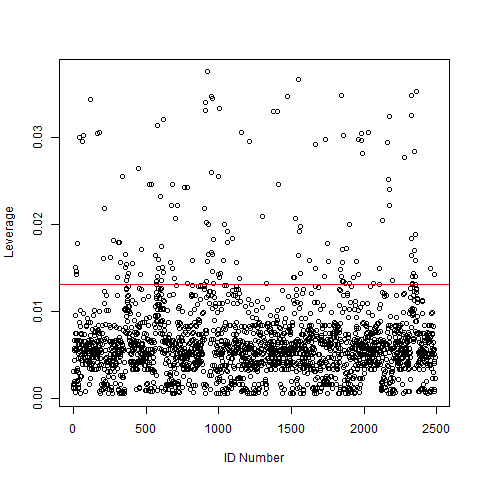
\includegraphics[width=\linewidth]{Leverage_of_logit.png} 
        \caption{Leverage by index plot.} 
        \label{fig:lev}
    \end{subfigure}%
    \hspace{0.45cm}
    \begin{subfigure}[t]{0.48\textwidth}
    \centering
        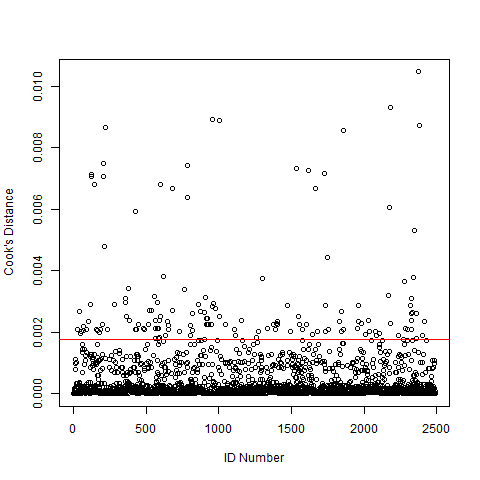
\includegraphics[width=\linewidth]{cook_for_logit.png} 
        \caption{Cook's distance by index plot.} \label{fig:cook}
    \end{subfigure}%
    
\caption{These plots depict the diagnostic testing results of the multiple logistic regression model.}
\label{fig:fig1}
\end{figure}
\graphicspath{{./images/}}
\begin{figure}[!htbp]
    \centering
    \begin{subfigure}[t]{0.48\textwidth}
    \centering
        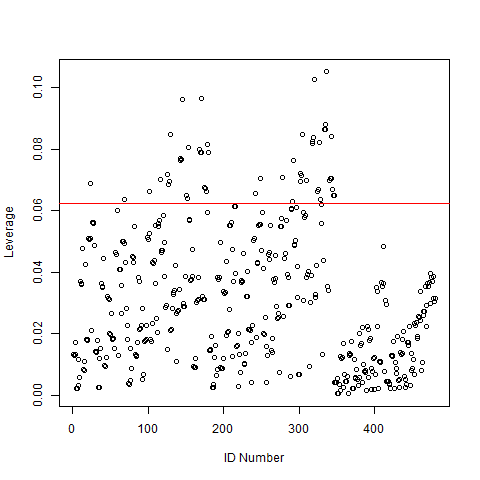
\includegraphics[width=\linewidth]{Leverage_for_poisson.png} 
        \caption{Leverage by index plot.} \label{fig:lev2}
    \end{subfigure}%
    \hspace{0.45cm}
    \begin{subfigure}[t]{0.48\textwidth}
    \centering
        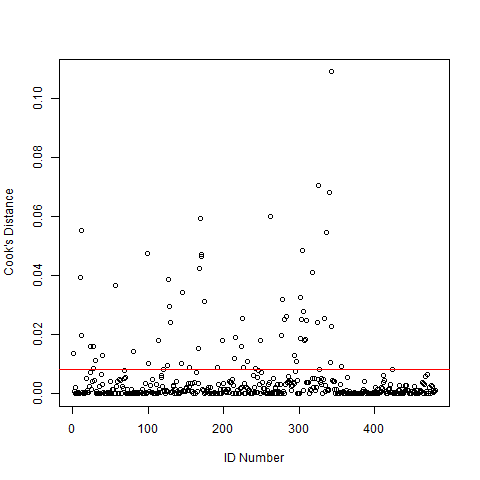
\includegraphics[width=\linewidth]{cook_for_poisson.png} 
        \caption{Cook's distance by index plot.} \label{fig:cook2}
    \end{subfigure}%
    
\caption{These plots depict the diagnostic testing results of the Poisson regression model.}
\label{fig:fig2}
\end{figure}
\newpage
% VIF
\begin{table}[!htbp]
\centering
\begin{longtable}[c]{@{}>{\raggedright\arraybackslash}p{23mm}>{\raggedright\arraybackslash}p{28mm}p{28mm}p{28mm}@{}}
\toprule
 & \textbf{GVIF} & \textbf{DF} & \textbf{GVIF\^(1/(2*Df))}\\* \midrule

 
\textbf{Urban} & 1.04 & 1 & 1.02 \\*  
\textbf{Sex} & 1.04 & 1 & 1.02  \\*  
\textbf{Age Group} & 1.50  & 3 & 1.07 \\*  
\textbf{Education} & 1.50 & 2 & 1.11 \\*  
\textbf{Occupation} & 1.07 & 1 & 1.04 \\*  
\textbf{Method} & 1.08 & 3 & 1.01 \\*  
\textbf{Season} & 1.03 & 3 & 1.01 \\* 

\bottomrule

\caption{VIF for the detection of presence of collinearity in the diagnostic testing of multiple logistic regression.}
\label{tab:T3}\\
\end{longtable}
\end{table}
% VIF
\begin{table}[!htbp]
\centering
\begin{longtable}[c]{@{}>{\raggedright\arraybackslash}p{45mm}>{\raggedright\arraybackslash}p{15mm}@{}}
\toprule
 & \textbf{VIF} \\* \midrule

 
\textbf{Residency: Urban} & 1.02  \\*  
\textbf{Sex: Male} & 1.02   \\*  
\textbf{Age Group: 35-49} & 2.22  \\*  
\textbf{Age Group: 50-64} & 2.91  \\*  
\textbf{Age Group: 65 and more} & 3.31  \\*  
\textbf{Education: Primary} & 1.60  \\*
\textbf{Education: Illiterate} & 1.63  \\*
\textbf{Occupation: Farming} & 1.02  \\*  
\textbf{Method: Other poison} & 1.01  \\*  
\textbf{Method: Hanging} & 1.06  \\*  
\textbf{Method: All others} & 1.03  \\*  
\textbf{Season: Autumn} & 1.47  \\* 
\textbf{Season: Winter} & 1.46  \\* 
\textbf{Season: Spring} & 1.52  \\* 


\bottomrule

\caption{VIF for the detection of presence of collinearity in the diagnostic testing of Poisson regression.}
\label{tab:T4}\\
\end{longtable}
\end{table}

\newpage
\section*{Conclusion}

In this study of fatality of suicide in a Chinese
population, factors including age group, education, occupation, method, and season are tested to be influential on the fatality rate after suicide in both models. People who are living in urban areas, who are male, who are older, who are with low education, or with a farmer occupation and who hung to suicide have higher fatality rates as shown in the result of multiple logistic regression. Unlike the result in multiple logistic regression, in the Poisson regression, however, people living in rural areas have a higher fatality rate after suicide, and people who hung, who suicide in autumn or winter have a lower fatality rate due to suicide. And sex difference seems to be not significant in the fatality rate in Poisson regression model. This study gives suggestions about the targets which should be focused on and provided suicide prevention. 

\newpage
\bibliographystyle{plain}
\bibliography{ref.bib}




\end{document}
